\begin{abstract}
\noindent
This paper measures how exposed workers are to generative AI in three
Sub-Saharan African economies, using household surveys that reach agricultural
and own-account workers and the own-use producers outside the employment
boundary. Across 24,838 workers
in Nigeria, Tanzania and Uganda the mean task-exposure score is 0.072, and
0.090 weighted, on the moderate 2030 Qwen 2.5 ratings, and runs 0.045 to
0.489 across nine versions. Agricultural workers average 0.029 against 0.134
for non-agricultural own-account workers and 0.150 for non-agricultural wage
employees. Inside wage work, formal employees average 0.213 against 0.104 for
informal ones. Clerical support, the most exposed major occupational group at
0.615, holds 0.6 percent of the sample. Giving employed workers a high-income
occupational mix, with their own occupation scores, raises exposure from 0.088
to 0.209.
\end{abstract}

\vspace{6pt}
\noindent\textbf{Keywords:} generative AI, occupational exposure, informality, structural transformation, Sub-Saharan Africa.

\noindent\textbf{JEL codes:} J21, J24, O33, O55.
\vspace{6pt}

\section{Introduction}

Generative-AI job exposure estimates are now available for many of the world's economies
\citep{felten2021,eloundou2024,gmyrek2023}, and all of them examine the people the statistical
system counts as employed. The 19th International Conference of Labour Statisticians resolved
that production mainly for a household's own use no longer counts as employment
\citep{icls2013}, and the survey data these studies examine follow that boundary. 
In the three
African economies examined here, own-use producers are a quarter of the workers in the
household surveys.

\citet{pizzinelli2023} score
worker-level microdata from labour force and household surveys in six
economies, counting formal, informal and self-employed workers alike.
\citet{cazzaniga2024} apply the same classification to 142 countries through the
ILO employment data. \citet{gmyrek2023} score 59 countries at four-digit
occupation codes, eight of them low income, and cascade the result up to global
and income-group aggregates, which \citet{gmyrek2025} refine on the same
harmonised microdata collection. None of the four splits wage jobs by
formality or counts own-use producers. \citet{demombynes2025} 
score four-digit worker data for 25 low- and middle-income countries,
Tanzania among them, and find self-employed and unpaid workers more exposed
than paid employees once occupation group and sector are held fixed.
\citet{gmyrek2024lac} split exposure by formality and employment status in
Latin America at two digits. This paper supplies the decomposition for
household-survey data from Sub-Saharan Africa and divides exposure between
agriculture, wage work and own-account work, splits wage jobs into formal and
informal, and shows how far the average moves once own-use producers are
counted.

This paper asks how exposed workers in three African economies are to generative
AI, how that exposure is spread across occupations and employment categories,
how much of the low average is a matter of where employment sits, and whether
the same structural patterns show up across a wider set of African economies.

To answer these questions I use the Living Standards Measurement Study
Integrated Surveys on Agriculture (LSMS-ISA), which records the main-job
occupation of working household members whether or not they work in the formal
economy \citep{lsmsisa}. I take the three LSMS-ISA waves that carry four-digit
occupation codes, for Nigeria (2023), Tanzania (2020) and Uganda (2019), link
each worker's occupation to a task-level measure of generative-AI capability
through an occupation crosswalk, and harmonise the result into a sample of
24,838 workers. A fourth wave, Ethiopia (2021), records only one-digit
occupation codes and enters as a supplement in Appendix~\ref{app:ethiopia}.

The evidence is descriptive and it shows that exposure is low and heavily 
concentrated on the
moderate 2030 ratings scored by Qwen 2.5, the measure's canonical version. The
pooled mean is 0.072 on a zero-to-one scale and 0.090 on survey weights. More
than half of all workers, 57.5 percent, score below 0.05, and the most exposed
tenth of workers holds 43 percent of the sum of worker exposure scores.
On the same measure, agricultural workers average 0.029 against 0.134 for
non-agricultural own-account workers and 0.150 for non-agricultural wage
employees. Clerical support work scores 0.615, nearly double the next group, 
and employs 0.6 percent of
the sample. The occupations generative AI is rated able to reach furthest into
by 2030 are the ones almost nobody in these economies works in.

Within non-agricultural wage employment, formal
workers score 0.213 and informal workers 0.104, and the gap holds in all three
countries. Agriculture sorts 62 percent of the
sample, and formality sorts inside the 17 percent who hold non-agricultural
wage jobs. The surveys ask the formality questions of wage employees alone,
which leaves own-account formality unmeasured.
A cross-section of African economies shows the same structure, with one
qualification the worker-level data help settle. Aggregate exposure falls as
informal employment and agricultural self-employment rise and climbs with income
per head. Which of the two carries the relationship depends on how aggregate
exposure is measured. Under a country measure built from occupation shares and
the worker-level scores estimated in this paper, the agricultural share does the work and
informality adds little once agriculture and income are held fixed.

These results add to the finding that low-income economies are less exposed to
AI \citep{pizzinelli2023,cazzaniga2024}. Once agricultural,
own-account and own-use workers are in the data, the low average reflects the
concentration of employment in occupations assigned low exposure. 
Giving these three economies the occupational mix
of the United Kingdom, and keeping their own occupation scores, raises exposure
from 0.088 to 0.209, with managers, professionals, technicians and clerical
support carrying the whole of that rise. Measured exposure differences follow
the task composition of the occupation, which is how the score is built. In
these three countries very few jobs contain the tasks a model is rated able to
do by 2030 under the moderate scenario.

What this paper adds is coverage and granularity as the sample holds 6,372
own-use producers, whom the employment boundary keeps out of the estimates
above, and it records work status, wage-job formality and the agricultural
split for each of the three countries on its own.

\subsection{Related literature}

Work measuring the exposure of jobs to automation and AI starts from the task
framework of \citet{autor2003} and \citet{acemoglu2019,acemoglu2022}, which
treats an occupation as a bundle of tasks and asks which of those tasks a
technology can carry out. That tradition runs from computerisation probabilities
\citep{frey2017} to AI occupational exposure scores \citep{felten2021,webb2020}
and large-language-model exposure \citep{eloundou2024}. I use the task-level
generative-AI measure of \citet{althoff2026}, which rates each O*NET task for
whether a language model will be able to perform it by 2030. This paper 
maps an existing measure onto household-survey
workers at a level of employment-status detail that existing cross-country
estimates do not provide, and it adds the own-use producers outside the
conventional employment boundary. A separate literature estimates realised effects of
generative AI on productivity and labour demand
\citep{brynjolfsson2023,noy2023,hui2023}, almost all of it in high-income or
online settings.

A parallel literature compares exposure across countries. \citet{alonso2020}
warn that AI may widen the gap between rich and poor economies.
\citet{pizzinelli2023,cazzaniga2024,gmyrek2023} find that low-income economies
are less exposed, given that fewer of their workers hold the occupations AI
reaches. \citet{gmyrek2025} refine the four-digit index and report global,
regional and income-group exposure through the same ILO estimation framework.
All of those routes measure employment as the labour force surveys define it.
The household surveys used here add the own-use producers that boundary leaves
out, and report the agricultural, own-account and informal structure country by
country.

Informality and structural transformation are the other body of work this paper
draws on. \citet{laporta2014} document how far informal and own-account work
dominates employment in low-income economies, and \citet{gollin2014} show how
much labour remains in low-productivity agriculture. I set those two facts
against the exposure measure and ask how much of the low African average they
account for.

\section{Data and measurement}

\subsection{What the exposure measure measures}

Throughout the paper, exposure means the importance-weighted share of
an occupation's tasks that a language model is rated able to perform.
\citet{althoff2026} rate every O*NET task on a four-point capability scale and
record the top two points as a yes-or-no rating. The occupation score is the
mean of that rating over the occupation's tasks, weighted by the O*NET importance
weight of each task. The result runs from 0
to 1. A score of 0.20 means that tasks carrying a fifth of the occupation's total
task importance are rated automatable.

The weight is an importance weight and a task can matter a
great deal to a job without filling much of the working day, and the score
therefore measures no share of time. The canonical ratings are also written
against a moderate 2030 scenario, which asks what a model will be able to do by
2030 under a middling rate of capability advance. The score describes the reach
of the technology over the next few years, and taking it as a description of
what models do at the time of writing would read it too high.

The level of exposure depends on which release of the ratings is used, and I
hold the release fixed at the version of 7 June 2026 published with
\citet{althoff2026}. Appendix~\ref{app:source} identifies each file exactly and
shows that the task ratings reproduce the published occupation scores.

Exposure is a property of the
job's task mix, and two workers in the same occupation receive the same score
whatever their skill or their employer. It describes what the technology can do 
and it is distinct from job loss. A task a model can perform may be automated,
may be handed to the model with the worker still doing the rest of the job, or
may go on being done by hand where nobody in that workplace has a reason or the
means to change. Adoption, electricity, connectivity, product-market competition
and the price of labour all sit between an exposure score and any labour-market
outcome, and none of them is measured here. Except where
Section~\ref{sec:cross} refers explicitly to the Global Automation Atlas, the
words automation exposure or AI exposure in this paper refer to this same
score.

The published measure comes in nine versions. Two models, Qwen 2.5 and
gpt-oss, are rated under four scenarios each, GPT-4o is rated under one and 
section~\ref{sec:measure} reports all nine. The headline uses the moderate
scenario scored by Qwen 2.5, the version the authors treat as canonical. The
choice moves the level of exposure. Four orderings hold across all nine.
Agriculture is the least exposed group in every version and far below both
non-agricultural groups, clerical support is the most exposed major group in
eight of the nine and second to managers in the ninth, formal wage employees
score above informal ones in every one, and Nigeria sits above the other two
in every one, within the coverage boundary Section~\ref{sec:addback} sets on
the distance between Uganda and Tanzania. Inside non-agricultural work, whether
wage or own-account sits higher moves with the version, and
Section~\ref{sec:measure} reports it.

\subsection{Surveys and occupation coding}

For each country I use the LSMS-ISA wave that carries coded occupations: the
General Household Survey Wave 5 for Nigeria, the National Panel Survey Round 5
for Tanzania, and the National Panel Survey for Uganda. Each records the
main-job occupation of working household members at the four-digit ISCO-08 unit
group \citep{isco08}. Ethiopia's Socioeconomic Panel Survey Wave 5 records only
the one-digit major group, too coarse to carry an occupational argument, and it
is reported separately in Appendix~\ref{app:ethiopia}.

Coverage of the occupation question differs across the three. In Uganda 7,671 of
the 7,688 people with a main-job record carry a four-digit code. Nigeria's
labour module carries a derived work-status variable, and that variable
settles who the coded workers are. Of the 7,656 people it records as
having worked in the last seven days, for pay, in a non-farm business or on the
farm for market, 7,591 carry a four-digit code and 65 do not. A further 117
coded workers report no work in the last seven days. The sample keeps all 117.
Of them, 115 expect to be back in a job within three months, which holds them
inside employment on the same definition; the other two are kept for
consistency with the survey's own coding, and dropping them moves no figure in
this paper at three decimals. Those two groups are the 7,708 coded Nigerian
workers in
Table~\ref{tab:flow}. A third group, the 1,839 people whose only work is on the
family farm, is asked no occupation question at all, and
Section~\ref{sec:sample} sets out how it enters.

For Tanzania, its labour module codes occupation
for non-farm jobs only, and farmers enter through the agricultural-labour
question. It codes a further 139 workers to the national TASCO classification, 
for which I found no
published correspondence to ISCO-08. And it asks no occupation at all of non-farm business
owners without a wage job, which removes 1,789 own-account workers from the
Tanzanian sample and means the pooled own-account figures rest on Nigeria and
Uganda. Sections~\ref{sec:sample} and \ref{sec:robust} take each of these apart.

\subsection{From O*NET tasks to survey workers}

The chain that carries an exposure score from a task rating to a worker in a
Ugandan village runs through four steps, and each loses some information.

\emph{Step 1, tasks to O*NET occupations.} Task ratings are aggregated to each
O*NET-SOC 2010 occupation with O*NET task weights, as described above.

\emph{Step 2, O*NET-SOC to SOC-2010.} O*NET-SOC detailed codes roll up to their
SOC-2010 base code. This step loses little, given that O*NET-SOC is a refinement
of SOC.

\emph{Step 3, SOC-2010 to ISCO-08.} I use the published ISCO-08 to SOC-2010
correspondence. Mapping is not one-to-one in either direction. Of the 423
ISCO-08 unit groups that receive a score, 127 map to a single O*NET-SOC
occupation and 296 map to more than one, with a median of two and a maximum of
35. Where an ISCO code maps to several O*NET occupations I take the unweighted
mean of their scores. The unweighted mean treats every O*NET occupation inside
an ISCO group as an equally plausible account of what an African worker in that
group does. It is a real assumption, and Section~\ref{sec:crosswalk} shows what
happens under five alternatives, including one that weights by US employment.
Seven codes appearing in the Nigerian data have no direct match. Six take the
average of their three-digit parent group and one takes its two-digit parent.

\emph{Step 4, ISCO-08 to the survey worker.} Workers merge on their four-digit
code. The 139 Tanzanian workers coded to TASCO are mapped to ISCO-08 by hand.
I found no published correspondence from TASCO to ISCO-08. TASCO adapts
ISCO-88, but 18 of the 19 codes involved are TASCO additions with no ISCO-88
counterpart, and the ILO's ISCO-88 to ISCO-08 table cannot place them. The map
was built from the job
descriptions the respondents themselves gave, and it is checked in
Section~\ref{sec:sample}. Of the 24,838 workers, 17,720 (71.3 percent) carry a
four-digit code. The other 7,118 are 6,372 family-use own-use farmers, who take
a subsistence score described below, 740 market-oriented Tanzanian farmers, who
take the major group 6 mean, and six TASCO rows scored above the four-digit
level.

\subsection{Harmonised variables}

For each worker I record age, sex, urban or rural residence, the four-digit
occupation and its ISCO major group, and an employment-status category.
Agricultural workers are those in ISCO major group 6 or in agricultural
elementary occupations, assigned from the occupation code. 
Everyone else splits into wage employees and
own-account workers using the main-job employer question in each survey. In
Uganda the question asks about the main job. Appendix~\ref{app:vars} lists
the survey variables used for every concept.
Employment status, occupation and the formality questions then all describe the
same job. The own-account category is a residual. It holds anyone who is not a wage
employee, including unpaid family workers and apprentices, and it should be read
as own-account and other.

I classify each wage job as formal or informal on a rule the three surveys can
all support. A wage job counts as informal when it comes with no written contract
and no second marker of formal status, which is pension coverage in Nigeria,
income-tax withholding in Tanzania and PAYE deduction in Uganda. This gives a
common two-part operational rule, though the second marker differs across
surveys. Tanzania
and Uganda carry fuller question sets, and Section~\ref{sec:who} reports what
those give. The formality split covers 4,267 wage workers in three countries.

\subsection{Building the estimation sample}
\label{sec:sample}

Two construction choices decide who counts as employed given that they move 
the pooled mean more than anything else in
the paper.
The first is own-use farmers, people who farm only to feed their own household.
The 19th International Conference of Labour Statisticians places them outside
employment \citep{icls2013}, and the ILOSTAT employment series used in
Section 6 follow that boundary. 
The LSMS-ISA surveys record them and excluding them would drop 6,372 workers, a quarter
of the sample, and would reproduce exactly the coverage gap this paper exists to
close. I keep them in the headline sample, give them the mean score of the four
ISCO subsistence-farming unit groups (6310, 6320, 6330 and 6340), which is
0.019, and report the sample without them throughout. The boundary turns on
the main intended destination of the output. Tanzania's survey asks it
directly, whether the products are intended only for sale, mainly for sale,
mainly for family use or only for family use. The 740 who answer only or
mainly for sale are market-oriented farmers who also keep some output. They
sit inside employment and take the broader ISCO major-6 average of 0.076.
Nigeria's labour module asks the same question in a different form, whether
farm output is only for sale, for sale and household use, or only for
household use, and if both, what share is sold. Its derived work-status
variable puts a person on the family farm only when that
farm is their sole work and its output is only or mainly for household use.
Mainly means a quarter or less is sold, or half with most kept. Of the 1,839,
985 sell nothing and 854 keep most of the output. For 24 with no farm work in
the reference week, the answer comes from the same questions asked about
usual farm work. All 1,839 are family-use own-use producers on the
same main-destination test applied in Tanzania.

The second is the treatment of the 1,789 Tanzanian non-farm business owners the
survey never asks about occupation. These workers cannot be scored at all and
are absent from the sample. The consequence is visible in
Table~\ref{tab:summary}, where Tanzania's own-account share is zero.
Section~\ref{sec:addback} puts them back under five imputation routes and
reports what that does to the country ordering.

Table~\ref{tab:flow} traces every worker from the household roster to the
estimation sample, with the reason for each drop.

\begin{table}[ht]
\centering
\caption{From the household roster to the estimation sample}
\label{tab:flow}
\small
\begin{tabular}{lrrr}
\toprule
Stage & Nigeria & Tanzania & Uganda \\
\midrule
Roster respondents                                   & 28{,}256 & 23{,}592 & 16{,}056 \\
Coded occupation, matched to exposure                & 7{,}708  & 2{,}208  & 7{,}671 \\
TASCO code mapped by hand                            &          & 139      &  \\
Market-oriented farmers                              &          & 740      &  \\
Own-use farmers, family use                          & 1{,}839  & 4{,}533  &  \\
\midrule
Estimation sample                                    & 9{,}547  & 7{,}620  & 7{,}671 \\
\midrule
Not recoverable: no occupation question asked        &          & 1{,}789  &  \\
\bottomrule
\end{tabular}

\vspace{4pt}
\begin{minipage}{0.92\linewidth}
\footnotesize
Market-oriented farmers, whose output is only or mainly for sale, take the
ISCO major-6 average of 0.076,
and family-use farmers take the subsistence-group average of 0.019. The final row
counts Tanzanian non-farm business owners without a wage job, whom the survey
never asks about occupation. The pooled sample is 24,838 workers.
\end{minipage}
\end{table}

Table~\ref{tab:summary} reports the sample and its survey-weighted counterpart.
The agricultural share runs from 42.2 percent in Nigeria to 76.5 percent in
Tanzania, and mean exposure moves against it.

\begin{table}[ht]
\centering
\caption{Sample composition, unweighted and survey-weighted}
\label{tab:summary}
\small
\begin{tabular}{lrrrrrrrr}
\toprule
 & & & & \multicolumn{2}{c}{\% agriculture} & \multicolumn{2}{c}{Mean exposure} \\
\cmidrule(lr){5-6}\cmidrule(lr){7-8}
Country & $N$ & \% female & Mean age & Sample & Weighted & Sample & Weighted \\
\midrule
Nigeria 2023  & 9{,}547  & 47.2 & 38.8 & 42.2 & 36.9 & 0.102 & 0.107 \\
Tanzania 2020 & 7{,}620  & 44.2 & 32.4 & 76.5 & 80.8 & 0.050 & 0.044 \\
Uganda 2019   & 7{,}671  & 49.7 & 33.4 & 72.8 & 64.9 & 0.055 & 0.068 \\
\midrule
All (pooled)  & 24{,}838 & 47.1 & 35.2 & 62.2 & 48.6 & 0.072 & 0.090 \\
\bottomrule
\end{tabular}

\vspace{4pt}
\begin{minipage}{0.92\linewidth}
\footnotesize
Mean exposure is the importance-weighted generative-AI score on a 0-1 scale.
$N$, \% female and mean age are unweighted. Sample
columns are unweighted shares of survey rows and are not population estimates.
Weights are the cross-sectional household weights supplied with each wave,
with complete coverage in all three. Appendix~\ref{app:vars} names them. Agriculture is
ISCO major group 6 plus agricultural elementary occupations.
\end{minipage}
\end{table}

\subsection{Weights, survey design and the pooled mean}

The paper reports weighted and unweighted figures because they answer different
questions. The unweighted mean describes the sample. The weighted mean is a
survey-weighted estimate for the analytical population each wave covers, which
is the working members of sampled households with a coded occupation. The
country estimates in Table~\ref{tab:summary} carry the population reading. The
pooled weighted figure combines three analytical samples taken in three
different years, Uganda in 2019, Tanzania in 2020 and Nigeria in 2023, and it
leaves out Tanzania's 1,789 non-farm business owners, whom the survey never
asks about occupation.

Country means move little between the two with Nigeria going from 0.102 to 0.107,
Tanzania from 0.050 to 0.044 and Uganda from 0.055 to 0.068. 
Pooling survey rows gives an agricultural share of 62.2
percent and a mean of 0.072. Applying weights and pooling gives 48.6 percent
and 0.090. That gap comes from Nigeria, whose population is far larger than
Tanzania's and Uganda's but whose sample is a similar size. Weighting therefore
shifts the pooled figure towards Nigeria's lower agricultural share and higher
exposure. A mean that weights the three countries
equally is 0.073.

The unweighted pooled statistics in this paper are described as sample
shares. The corresponding population statement for the
agricultural share is 48.6 percent across the three countries, and the
country-by-country weighted estimates in Table~\ref{tab:summary} are reported 
for each of the countries. Exposure
is low and graded steeply by occupation under either treatment, and the country
ranking is the same: Nigeria, then Uganda, then Tanzania.

All three surveys are stratified multi-stage samples, and the intervals
reported below account for stratification and clustering by primary sampling
unit (PSU). Intervals around
unweighted sample means do not turn those means into population estimates. The
term population estimate is kept for the weighted figures. 
Nigeria and Tanzania supply cluster and stratum codes
directly. Uganda supplies neither, and the parish stands in for the enumeration
area, which is the identifier any household file carries.
Appendix~\ref{app:design} gives the design per country and shows what the
substitution costs. 
Standard errors that allow for strata and clusters run from 0.96 to 1.55 times
their household-clustered counterparts, and the ratio is largest for groups 
whose members share villages.

\section{How much exposure, and where}

The pooled sample mean is 0.072, with a 95 percent interval of 0.069 to 0.074.
The weighted population estimate is 0.090. 
Either way the average worker in these three
countries holds a job in which well under a tenth of the task importance sits in
tasks a language model is rated able to perform. 
More than half of all workers, 57.5
percent, score below 0.05, which is close to nothing, and 68.5 percent work in
agricultural or elementary occupations. The most exposed tenth of workers
holds 43 percent of the sum of worker exposure scores, unweighted.

Table~\ref{tab:major} reports worker shares and mean exposure by ISCO major
group. The gradient is steep and it runs along familiar white-collar lines. 
Clerical support work sits above everything else as its mean
of 0.615 is nearly double the next group, technicians at 0.363, and about twenty
times the score for skilled agriculture. This fits what is already known about
large language models as they are at their strongest on text, records,
correspondence, scheduling and routine information handling, which is close to a
full description of clerical work. \citet{eloundou2024} find the same peak in US
data.

Clerical support
holds 0.6 percent of the pooled sample. Technicians add 1.6 percent. 
The two are the most exposed groups and account for 2.2 percent of the workers. 
Skilled agriculture, at 0.031, holds 57.8 percent of the sample, and elementary
occupations, the least exposed group at 0.028, hold another 10.7 percent.
Figure~\ref{fig:gradient} sets the two columns side by side. 
Every group with a long exposure bar has a short worker bar,
and the one group that fills the worker panel sits at the bottom of the
exposure panel. The occupations generative AI reaches furthest into are the
occupations these economies barely have and that is the mechanism behind the low
average.

\begin{table}[ht]
\centering
\caption{Worker share and mean generative-AI exposure by ISCO major group}
\label{tab:major}
\small
\begin{tabular}{lrrr}
\toprule
ISCO major group & Share of workers & Mean exposure & 95\% interval \\
\midrule
Clerical support             & 0.6\%  & 0.615 & [0.590, 0.639] \\
Technicians and associates   & 1.6\%  & 0.363 & [0.339, 0.388] \\
Managers                     & 4.8\%  & 0.209 & [0.204, 0.215] \\
Professionals                & 4.6\%  & 0.161 & [0.151, 0.170] \\
Plant and machine operators  & 3.4\%  & 0.144 & [0.138, 0.149] \\
Service and sales            & 11.5\% & 0.142 & [0.138, 0.147] \\
Craft and trades             & 5.0\%  & 0.051 & [0.046, 0.056] \\
Skilled agriculture          & 57.8\% & 0.031 & [0.030, 0.032] \\
Elementary occupations       & 10.7\% & 0.028 & [0.026, 0.030] \\
\bottomrule
\end{tabular}

\vspace{4pt}
\begin{minipage}{0.9\linewidth}
\footnotesize
Rows are sorted by mean exposure. Shares are of all 24,838 pooled workers,
including 7,112 farmers without a directly coded four-digit occupation, all in
major group 6. Of these, 6,372 are family-use own-use producers and 740 are
market-oriented Tanzanian farmers. Intervals are 95 percent and account for
stratification and PSU clustering. The means are unweighted, and the intervals
do not make them population estimates.
\end{minipage}
\end{table}

\begin{figure}[ht]
\centering
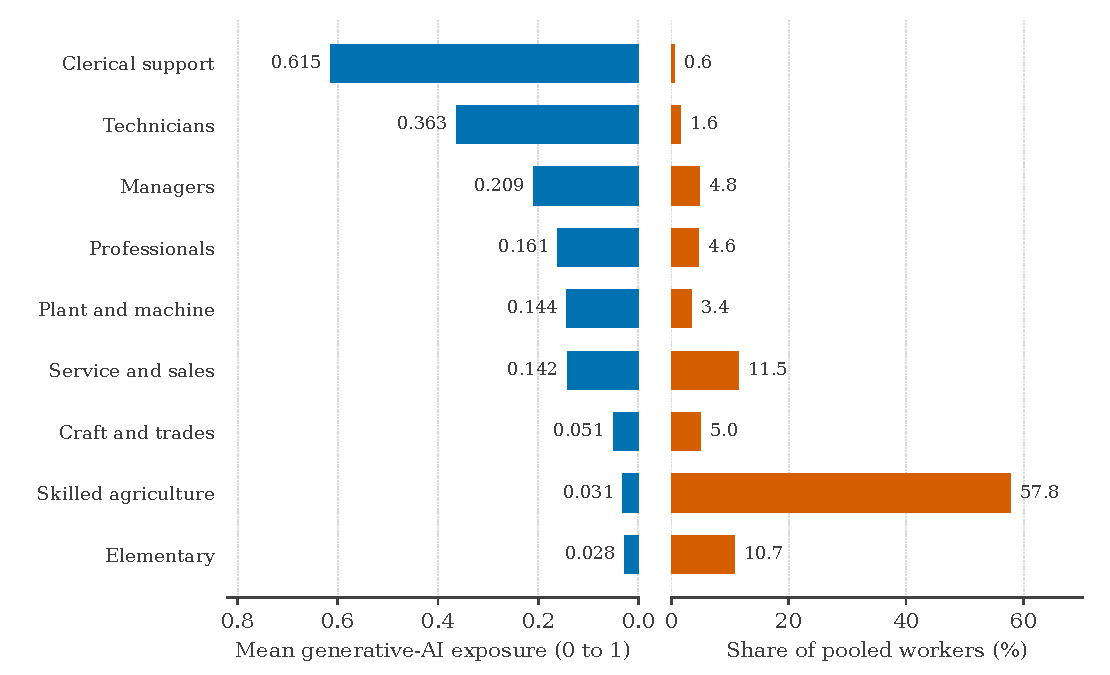
\includegraphics[width=0.86\linewidth]{figures/fig_occupation_gradient}
\caption{Mean generative-AI exposure and share of workers by ISCO major
group, pooled sample, ordered by exposure. The most exposed major groups hold
the smallest shares of workers.}
\label{fig:gradient}
\end{figure}

\section{Who is exposed}
\label{sec:who}

Table~\ref{tab:status} splits the sample by work status. Agriculture sits
at 0.029. Non-agricultural own-account workers
average 0.134 and non-agricultural wage employees 0.150. Estimated directly, the
wage premium over own-account work is 0.016 with a standard error of 0.004, and
0.033 with a standard error of 0.005 once country fixed effects absorb the
different country mixes. Both are far from zero and both are small next to the
gap of about 0.11 that separates either group from agriculture. On the weighted
basis the ordering is the same.

\begin{table}[ht]
\centering
\caption{Worker share and mean generative-AI exposure by work status}
\label{tab:status}
\small
\begin{tabular}{lrrrr}
\toprule
Work status & Share of workers & Mean exposure & 95\% interval & Weighted \\
\midrule
Agriculture                       & 62.2\% & 0.029 & [0.028, 0.031] & 0.037 \\
Own-account, non-agriculture      & 20.6\% & 0.134 & [0.130, 0.138] & 0.128 \\
Wage employee, non-agriculture    & 17.2\% & 0.150 & [0.144, 0.156] & 0.169 \\
\bottomrule
\end{tabular}

\vspace{4pt}
\begin{minipage}{0.9\linewidth}
\footnotesize
Agriculture is assigned from the occupation code. The remaining workers split on
the survey's main-job employer question, with own-account as the residual
category. Tanzania contributes no own-account workers, as its survey asks no
occupation of non-farm business owners, so that row rests on Nigeria and Uganda.
Intervals are 95 percent and account for the survey design.
\end{minipage}
\end{table}

The surveys put the formality questions to wage employees only,
which leaves the share of own-account workers who are informal unmeasured. Under
the ILO definition an own-account worker counts as informal when the enterprise
does, and status on its own settles nothing \citep{icls2023}. What the data do
say is that non-agricultural own-account workers score 0.134, close to wage
employees and well above farmers. The measured distance between a subsistence
farmer and everyone else comes from the task content the measure assigns to
farming, and the presence of a contract plays no part in it.

The formality question sharpens this. Within non-agricultural wage employment,
workers with no written contract and no second marker of formal status average
0.104, while formal wage workers average 0.213. Estimated directly on wage
workers with country fixed effects, the informal-formal contrast is $-0.102$
with a standard error of 0.006. Formal wage workers are about twice as exposed
as informal ones, and the pattern holds in all three countries, with
0.234 against 0.121 in Nigeria, 0.196 against 0.097 in Tanzania and 0.194
against 0.102 in Uganda. Formality therefore carries a strong signal inside wage
work. Measured informality among wage workers is 40.4 percent in Nigeria, 67.3
percent in Tanzania and 65.4 percent in Uganda. Where a country's survey
supports a fuller rule the level shifts and the exposure gap holds. Tanzania
reads 81.3 percent informal on the tax question alone, and Uganda 64.7 percent
on contract, pension and PAYE together.

Two divides therefore run through these labour markets, and per worker they are
much the same size. Agriculture sits 0.121 below non-agricultural wage
employment. Formal wage work sits 0.109 above informal wage work. What separates
the two divides is reach as the agricultural one sorts 15,441 workers, 62.2
percent of the sample, onto the low side. The formality one operates inside
non-agricultural wage employment, 17.2 percent of the sample, and only 1,801
workers sit on its formal side. Agriculture is what holds the aggregate down,
while formality is a steep gradient across a thin slice. Treating agriculture,
own-account work and informality as one undifferentiated low-exposure mass would
miss the second divide entirely.

Urban workers average 0.120 against
0.055 for rural workers, a gap of 0.064 that is wide in every country and that
survives country fixed effects at 0.062. Men average 0.077 and women 0.066. The
sex difference is estimated and small. At 0.011 it is a sixth of the
urban-rural gap and a tenth of the agricultural gap.

Table~\ref{tab:reg} puts these differences in one place and asks how much of
each is composition across countries. Column 1 is the raw status comparison.
Column 2 adds country fixed effects, and column 3 adds residence, sex and age.
The status gaps narrow a little and survive. Relative to agriculture,
own-account work carries 0.088 more exposure and wage employment 0.111 more,
with country, residence, sex and age held fixed. Figure~\ref{fig:ci} shows every
group mean with its interval.

\begin{table}[ht]
\centering
\caption{Generative-AI exposure and work status}
\label{tab:reg}
\small
\begin{tabular}{lccc}
\toprule
 & (1) & (2) & (3) \\
\midrule
Own-account, non-agriculture   & 0.105$^{***}$ & 0.093$^{***}$ & 0.088$^{***}$ \\
                               & (0.002) & (0.003) & (0.003) \\
Wage employee, non-agriculture & 0.121$^{***}$ & 0.120$^{***}$ & 0.111$^{***}$ \\
                               & (0.003) & (0.003) & (0.003) \\
Urban                          &         &         & 0.015$^{***}$ \\
                               &         &         & (0.002) \\
Female                         &         &         & $-0.005^{***}$ \\
                               &         &         & (0.001) \\
Age                            &         &         & 0.0003$^{***}$ \\
                               &         &         & (0.00005) \\
\midrule
Country fixed effects          &         & $\checkmark$ & $\checkmark$ \\
Observations                   & 24{,}838 & 24{,}838 & 24{,}838 \\
$R^2$                          & 0.270   & 0.277   & 0.285 \\
\bottomrule
\end{tabular}

\vspace{4pt}
\begin{minipage}{0.9\linewidth}
\footnotesize
Ordinary least squares. The dependent variable is the worker's generative-AI
exposure score. Agriculture is the omitted status. Regressions are unweighted
and describe conditional relationships in the analytical sample. Weighted by
the survey expansion weights, column (2) gives 0.080 (0.003) for own-account
and 0.129 (0.006) for wage work. Standard errors in
parentheses account for the stratified multi-stage survey design. In the
matching regression run on wage workers alone, informal status carries $-0.102$
(0.006) with country fixed effects. $^{*}p<0.1$, $^{**}p<0.05$, $^{***}p<0.01$.
\end{minipage}
\end{table}

\begin{figure}[ht]
\centering
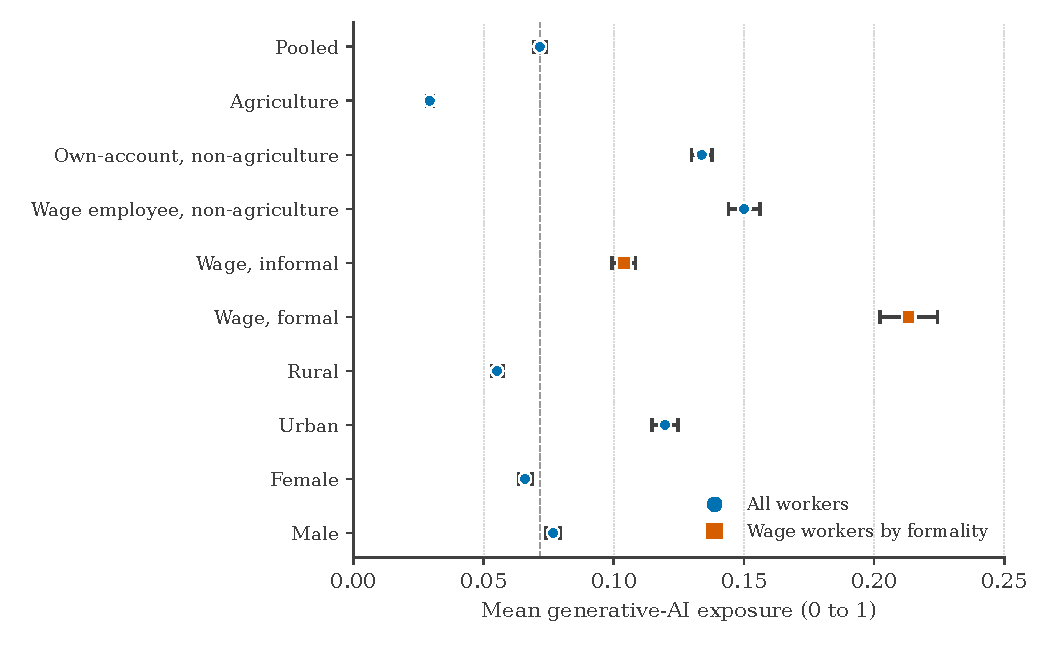
\includegraphics[width=0.86\linewidth]{figures/fig_group_means_ci}
\caption{Mean generative-AI exposure by group, with 95 percent intervals
accounting for the survey design. Most intervals are narrower than the marker.
The dashed line is the pooled mean.}
\label{fig:ci}
\end{figure}

\section{Robustness}
\label{sec:robust}

Three features of the construction could carry the results on their own: which
workers count as employed, the unweighted mean used when an ISCO code maps to
several O*NET occupations, and the choice among the nine published versions of
the exposure measure. This section tests each.

\subsection{The sample definition}

Table~\ref{tab:robust} recomputes the headline figures on four samples. The
strict column keeps the workers whose occupation came from the survey's own
coding, 17,726 in all. Of these, 17,720 carry a four-digit ISCO-08 code; six
are Tanzanian TASCO rows mapped to a sub-major group, which scores them
without giving them a unit code.

Leaving out the family-use own-use farmers, which is what the ILO employment
boundary implies, raises the pooled mean from 0.072 to 0.090 and cuts the
agricultural share from 62.2 to 49.1 percent. Keeping only coded occupations
gives almost the same figures. Dropping the 139 hand-mapped TASCO rows moves the
pooled mean by 0.001. The occupational gradient, which is the paper's result, is
untouched in every column, where the two non-agricultural status means are
identical to three decimals throughout, as none of the affected workers is in
them.

\begin{table}[ht]
\centering
\caption{Robustness to the sample definition}
\label{tab:robust}
\small
\begin{tabular}{lrrrr}
\toprule
 & Headline & Family-use & Coded & TASCO rows \\
 &          & farmers out & occupations only & left out \\
\midrule
Workers                        & 24{,}838 & 18{,}466 & 17{,}726 & 24{,}699 \\
Mean exposure                  & 0.072 & 0.090 & 0.090 & 0.071 \\
Mean exposure, weighted        & 0.090 & 0.110 & 0.111 & 0.090 \\
\% agriculture                 & 62.2  & 49.1  & 47.0  & 62.5 \\
\% scoring below 0.05          & 57.5  & 42.8  & 44.6  & 57.8 \\
Agriculture, mean              & 0.029 & 0.037 & 0.033 & 0.029 \\
Own-account non-agric., mean   & 0.134 & 0.134 & 0.134 & 0.134 \\
Wage non-agric., mean          & 0.150 & 0.150 & 0.150 & 0.151 \\
\bottomrule
\end{tabular}

\vspace{4pt}
\begin{minipage}{0.9\linewidth}
\footnotesize
The second column applies the ILO employment boundary \citep{icls2013} by
dropping the 6,372 family-use own-use farmers and keeping Tanzania's 740
market-oriented farmers. The third keeps only workers with a directly coded
four-digit occupation. The fourth drops the 139 Tanzanian workers whose TASCO
codes were mapped to ISCO-08 by hand.
\end{minipage}
\end{table}

The score given to the own-use farmers deserves a test of its own, as it sets
the exposure of a quarter of the sample. In the headline the 6,372
family-use farmers receive 0.019, the average of the four ISCO subsistence
unit groups. Table~\ref{tab:imputed} recomputes the pooled mean under four
alternatives, from zero to the highest-scoring major-6 occupation.
The pooled level does depend on this choice and the
ranking of groups does not. At every value, agriculture stays far below both
non-agricultural groups, and the full range of defensible pooled means, 0.067 to
0.093, leaves the pooled mean below a tenth throughout.

\begin{table}[ht]
\centering
\caption{Pooled exposure under alternative scores for the own-use farmers}
\label{tab:imputed}
\footnotesize
\begin{tabular}{llrrr}
\toprule
Score & Source & Pooled mean & Weighted & Agriculture mean \\
\midrule
0.000 & Lowest major-6 code       & 0.067 & 0.086 & 0.022 \\
0.019 & Subsistence groups (headline) & 0.072 & 0.090 & 0.029 \\
0.076 & Major-6 average           & 0.086 & 0.103 & 0.053 \\
0.102 & Highest major-6 code      & 0.093 & 0.109 & 0.063 \\
\bottomrule
\end{tabular}

\vspace{4pt}
\begin{minipage}{0.9\linewidth}
\footnotesize
The score is applied to the 6,372 family-use own-use farmers in Nigeria and
Tanzania. Changing the score of Tanzania's 740 market-oriented farmers moves 
the pooled mean by about 0.002 at most.
\end{minipage}
\end{table}

\subsection{Tanzania's uncounted business owners}
\label{sec:addback}

Tanzania's survey asks no occupation of 1,789 non-farm
business owners, who therefore carry no score and sit outside the estimation
sample, which is why Tanzania's own-account share in Table~\ref{tab:summary} is
zero. The missing workers all belong to the country at the bottom of the
ranking, and none of the tests above can see them.

Table~\ref{tab:addback} puts them back. Each of the 1,789 carries its own
household expansion weight, joined from the file the rest of the Tanzanian
sample already uses, and averaging 2,628 against a Tanzanian mean of 2,736.
Four flat scores bound the answer: zero, the agricultural mean of 0.029, the
own-account non-agricultural mean of 0.128 and the wage non-agricultural mean
of 0.169. A fifth route scores them by industry. Of the 1,789, 1,555 (87.1
percent) link to a household enterprise carrying an ISIC section code, and each
takes the weighted mean exposure of Ugandan non-agricultural own-account
workers in the same section. That route implies 0.162, inside the flat range.
These workers stay out of the headline sample, since any score given to them is
an assumption.

The pooled mean barely moves, from 0.087 at a score of zero
to 0.093 at the highest imputation, against a headline of 0.090. Tanzania
stays below Uganda at every score, while the margin closes. At zero it is 0.033.
At the wage non-agricultural mean it is 0.001, and the two countries' 95 percent
design-based intervals overlap. The industry route does the same.
The country order Nigeria, Uganda, Tanzania therefore holds as a ranking of
point estimates under every crosswalk rule, in all nine rating versions and
against this add-back. The distance between Uganda and Tanzania is smaller
than the coverage gap in one of them, and what this paper takes from the
cross-country comparison is Nigeria's distance from the other two.

\begin{table}[ht]
\centering
\caption{Adding Tanzania's 1,789 uncounted business owners back}
\label{tab:addback}
\footnotesize
\begin{tabular}{llrrlr}
\toprule
Score & Source & Pooled, & Tanzania, & Tanzania, & Margin over \\
      &        & weighted & weighted & 95\% interval & Uganda \\
\midrule
0.000 & Zero                      & 0.087 & 0.036 & 0.033--0.038 & 0.033 \\
0.029 & Agriculture mean          & 0.088 & 0.041 & 0.039--0.043 & 0.027 \\
0.128 & Own-account non-agric.    & 0.092 & 0.059 & 0.056--0.062 & 0.009 \\
0.169 & Wage non-agric.           & 0.093 & 0.067 & 0.063--0.070 & 0.001 \\
0.162 & Industry match            & 0.093 & 0.065 & 0.062--0.068 & 0.003 \\
\bottomrule
\end{tabular}

\vspace{4pt}
\begin{minipage}{0.94\linewidth}
\footnotesize
Each of the 1,789 carries its own household expansion weight. Uganda's weighted
mean is 0.068, with a 95 percent interval of 0.063 to 0.073, and is the same in
every row. Intervals are design-based, with strata and primary sampling units
rebuilt from the Tanzanian household roster. The margin is Uganda's weighted
mean less Tanzania's. In the last two rows the two intervals overlap. Giving
the 1,789 the mean Tanzanian weight instead of their own moves every figure in
the table by 0.001 at most.
\end{minipage}
\end{table}

\subsection{The crosswalk aggregation}
\label{sec:crosswalk}

The unweighted mean over O*NET occupations within an ISCO group is the other
consequential choice. Table~\ref{tab:crosswalk} recomputes the headline figures
under five alternatives: the median, the minimum and the maximum of the linked
scores, a mean weighted by US employment, and 2,000 draws that pick one linked
occupation per ISCO code at random.

The employment weights come from the BLS Occupational Employment and Wage
Statistics for May 2018 \citep{oews2018}, the last release coded to the 2010
SOC and therefore the one that matches the crosswalk. They reach 422 of the 423
ISCO codes. This alternative answers a fair objection to the unweighted mean,
which is that O*NET subdivides some SOC occupations into several detailed codes
and leaves others whole, letting an arbitrary filing decision move the average. It
also imports the US occupational size distribution into an African measure,
which is why it appears here as an alternative.

Individual clerical ISCO codes run from 0.149 to
0.858, against a group mean of 0.615, the group average is taken over codes
that differ widely. The alternatives in Table~\ref{tab:crosswalk} nonetheless
leave the clerical mean between 0.543 and 0.684, a narrower proportional range
than agriculture's. The size of the clerical peak should be treated as
approximate and its position at the top of the distribution is somewhat secure.

Clerical support stays between 0.54 and
0.68, and at least thirteen times the skilled-agriculture score. The country
order is Nigeria, Uganda, Tanzania, and the draws' 95 percent ranges for the
three countries do not overlap. Agriculture is the least exposed group. The
separation of Uganda from Tanzania carries a boundary these draws cannot see,
and Section~\ref{sec:addback} states it.

The formality gap inside wage work holds under every rule as well. It stays
between 0.094 and 0.120 at the extreme bounds, and formal employees score above
informal ones in every one of the 2,000 draws.
The level shifts by about a third either way at the bounds, and
across the draws the pooled weighted mean has a standard deviation of 0.005,
more than twice its sampling standard error. And the wage premium over
own-account work, already the smallest gap in the paper, falls to zero at the
minimum, though wage workers score higher in 99.3 percent of draws and the
employment-weighted rule widens the gap to 0.020. That contrast is the least
secure result reported here, and Section~\ref{sec:measure} gives a second reason
to treat it with care.

\begin{table}[ht]
\centering
\caption{Sensitivity to the ISCO-to-O*NET aggregation rule}
\label{tab:crosswalk}
\footnotesize
\begin{tabular}{lrrrrrr}
\toprule
 & Mean & Emp. & Median & Min. & Max. & Draws, 95\% \\
 & (headline) & weighted &  &  &  & range \\
\midrule
Pooled, weighted        & 0.090 & 0.080 & 0.089 & 0.058 & 0.126 & 0.081--0.100 \\
Nigeria, weighted       & 0.107 & 0.095 & 0.106 & 0.070 & 0.147 & 0.095--0.118 \\
Uganda, weighted        & 0.068 & 0.057 & 0.066 & 0.042 & 0.098 & 0.058--0.078 \\
Tanzania, weighted      & 0.044 & 0.041 & 0.041 & 0.024 & 0.068 & 0.036--0.053 \\
Agriculture             & 0.029 & 0.020 & 0.029 & 0.008 & 0.050 & 0.018--0.041 \\
Own-account non-agric.  & 0.134 & 0.126 & 0.130 & 0.105 & 0.169 & 0.121--0.147 \\
Wage non-agric.         & 0.150 & 0.146 & 0.146 & 0.106 & 0.206 & 0.138--0.164 \\
Wage minus own-account  & 0.016 & 0.020 & 0.016 & 0.000 & 0.036 & 0.003--0.029 \\
Clerical support        & 0.615 & 0.613 & 0.617 & 0.543 & 0.684 & 0.568--0.661 \\
Skilled agriculture     & 0.031 & 0.021 & 0.031 & 0.008 & 0.053 & 0.019--0.044 \\
\midrule
Wage, formal            & 0.213 & 0.206 & 0.211 & 0.160 & 0.275 & 0.198--0.229 \\
Wage, informal          & 0.104 & 0.102 & 0.098 & 0.066 & 0.155 & 0.090--0.120 \\
Formal minus informal   & 0.109 & 0.104 & 0.113 & 0.094 & 0.120 & 0.096--0.124 \\
\bottomrule
\end{tabular}

\vspace{4pt}
\begin{minipage}{0.94\linewidth}
\footnotesize
Minimum and maximum are extreme bounds in which every ISCO code takes its lowest
or highest linked score at once. Group means are unweighted unless marked.
Employment weights are US national employment from \citet{oews2018}, applied at
the 6-digit SOC level and split evenly among the O*NET codes in each base; they
reach 422 of the 423 ISCO codes, and the remaining code keeps the simple mean.
The draws pick one linked O*NET occupation per ISCO code at random, 2,000 times.
The last three rows rest on the 4,267 wage workers whose formality status is
observed, a smaller base than the rows above them.
\end{minipage}
\end{table}

\subsection{The exposure measure}
\label{sec:measure}

\citet{althoff2026} publish nine versions of the task ratings. Two models,
Qwen 2.5 and gpt-oss, are rated under four scenarios each, and GPT-4o is
rated under one. Table~\ref{tab:variants} rescores every worker under each.

The structure survives all nine. The country order is Nigeria, Uganda, Tanzania
in every one, weighted and unweighted, within the boundary
Section~\ref{sec:addback} sets on the distance between Uganda and Tanzania.
Agriculture is the least exposed
employment group in every one. Clerical support is the most exposed major group
in eight of the nine, and in the ninth it is second to managers. Formal wage
employees score above informal ones in every one, by 0.067 to 0.155. Rank
correlations with the headline run from 0.80 to 0.96 across the 430 ISCO codes.

The pooled
weighted mean runs from 0.045 to 0.489 across the nine. The model matters as
much as the scenario. Under every scenario gpt-oss gives a higher pooled mean
than Qwen. The share of workers scoring below 0.05 runs from 0.1 percent to 71.6
percent. The level of exposure, and about
how many workers sit near zero reported in this study, belongs to the 
moderate Qwen scenario. The occupational gradient and the gap between
agriculture and both non-agricultural groups hold across all nine, and neither
depends on it.

Wage workers score above own-account workers under three of the nine
versions, and own-account workers score higher under the other six, by up to
0.114.  With the crosswalk bounds in Section~\ref{sec:crosswalk}, we
conclude that non-agricultural wage and own-account work are close together
and far above agriculture.

\begin{table}[ht]
\centering
\caption{Exposure under the nine published versions of the task ratings}
\label{tab:variants}
\footnotesize
\setlength{\tabcolsep}{4pt}
\begin{tabular}{llrrrrrrr}
\toprule
Model & Scenario & Rank & Pooled, & Agri- & Own- & Wage & Clerical & Formal \\
      &          & corr. & weighted & culture & account &      &  & less informal \\
\midrule
Qwen 2.5 & Moderate (headline) & 1.00 & 0.090 & 0.029 & 0.134 & 0.150 & 0.615 & 0.109 \\
gpt-oss  & Moderate            & 0.84 & 0.256 & 0.215 & 0.283 & 0.275 & 0.686 & 0.074 \\
Qwen 2.5 & Slow                & 0.94 & 0.045 & 0.011 & 0.066 & 0.085 & 0.409 & 0.081 \\
gpt-oss  & Slow                & 0.88 & 0.195 & 0.149 & 0.243 & 0.219 & 0.650 & 0.094 \\
Qwen 2.5 & Rapid               & 0.96 & 0.200 & 0.082 & 0.325 & 0.263 & 0.784 & 0.155 \\
gpt-oss  & Rapid               & 0.83 & 0.489 & 0.384 & 0.602 & 0.488 & 0.790 & 0.143 \\
Qwen 2.5 & No scenario         & 0.96 & 0.061 & 0.013 & 0.094 & 0.117 & 0.473 & 0.105 \\
gpt-oss  & No scenario         & 0.80 & 0.103 & 0.057 & 0.143 & 0.124 & 0.474 & 0.067 \\
GPT-4o   & No scenario         & 0.87 & 0.117 & 0.058 & 0.167 & 0.148 & 0.551 & 0.086 \\
\bottomrule
\end{tabular}

\vspace{4pt}
\begin{minipage}{0.94\linewidth}
\footnotesize
Rank correlation is with the headline scores across the 430 ISCO-08 codes.
Group means are unweighted. Every version is rescored through the same
task-to-occupation and occupation-to-ISCO rules as the headline. The scenario
sets how fast the rater assumes model capability advances. The last column is
the formal wage mean less the informal wage mean, and rests on the 4,267 wage
workers whose formality status is observed, a smaller base than the other
columns.
\end{minipage}
\end{table}

\section{From within-country to cross-country}
\label{sec:cross}

The within-country evidence document that exposure is low because of what 
workers do, but how much of the low exposure the occupational mix has on its own 
outside the three countries.
In Table~\ref{tab:composition}, the exposure score attached to each ISCO
major group is held at the value these three surveys imply, and the employment
shares are swapped for a high-income country's. The shares come from ILOSTAT
for the United Kingdom, Germany and France, each of which reports ISCO-08 with
under 2 percent of employment unclassified. In the third column, 
its score vector drops the family-use own-use farmers, so the scores and the
ILOSTAT shares describe the same employed population. On this construction the
three economies studied in the paper average 0.088. The United Kingdom's mix raises
that to 0.209, Germany's to 0.227 and France's to 0.203. The average African
country moves from 0.104 to 0.209 on the United Kingdom's mix. The full-sample
survey scores give 0.080 to 0.208, the crosswalk scores give the same pattern
at a higher level, and the three benchmarks agree.

The full-sample baseline of 0.080 differs from the headline weighted mean of 0.090, and the
whole of the difference is the source of the employment shares. The table needs
a share for all nine major groups in every country, including the benchmarks.
Only ILOSTAT covers all of them, and the table uses it throughout. Aggregation
adds nothing to the gap. Each group's score is itself the weighted mean of the
worker scores inside it. Applying the survey's own major-group shares to the
same score vector returns 0.090 exactly, to the tenth decimal. What moves the number is that
ILOSTAT and the surveys place workers in different groups. ILOSTAT puts 0.7
percent of these three countries' employment in major group 1 against 8.2
percent in this sample, which on its own accounts for $-0.015$ of the
$-0.011$ difference, and service and sales runs the other way, 23.3 percent
against 15.8 percent, for $+0.009$. Every other group contributes under 0.004.
Major group 1 in this sample is 1,202 workers, 89 percent of them own-account
and non-agricultural by weight, and 72 percent of that weight sits in one unit
code, retail and wholesale trade managers. The gap is about where a shopkeeper
is coded.

Group by group, the rise sits at the top of the occupational distribution. For
the average African country, managers, professionals, technicians and clerical
support together contribute 0.133 to the rise from 0.104 to 0.209, and the
smaller share in skilled agriculture takes 0.021 of it back. The gain comes
from the jobs a high-income workforce holds. Agriculture's retreat works the
other way, since those workers carried a score close to zero to begin with.

Changing nothing but where people work more than doubles exposure and that is the
size of the composition result.
The exercise holds the occupation scores fixed, such that it says what the mix does and
leaves open whether the same occupation has the same tasks in a rich
country. It also gives no share of the gap between these economies and a
high-income one, since the benchmark's exposure under its own occupation scores
is not estimated. And the
counterfactual level, about a fifth, still sits far below the clerical figure of
0.615, so a high-income mix moves these economies a long way up a distribution
whose top most workers never reach.

\begin{table}[ht]
\centering
\caption{Exposure under a high-income occupational mix}
\label{tab:composition}
\small
\begin{tabular}{lrrr}
\toprule
 & Crosswalk & Survey & Survey scores, \\
Occupational mix & mean scores & scores & own-use out \\
\midrule
These three economies, own mix   & 0.113 & 0.080 & 0.088 \\
Average African country, own mix & 0.133 & 0.098 & 0.104 \\
\midrule
United Kingdom                   & 0.261 & 0.208 & 0.209 \\
Germany                          & 0.256 & 0.227 & 0.227 \\
France                           & 0.242 & 0.203 & 0.203 \\
\bottomrule
\end{tabular}

\vspace{4pt}
\begin{minipage}{0.94\linewidth}
\footnotesize
Each cell is the sum over ISCO major groups 1 to 9 of an employment share times
a group exposure score. The score vector is held fixed down each column and the
employment shares change down the rows. Crosswalk mean scores average the
O*NET-linked score over the ISCO codes in each major group. Survey scores are
the weight-averaged worker scores estimated here. The third column, the
headline, drops the family-use own-use farmers from the score vector, matching
the ILO employment boundary the ILOSTAT shares follow. Employment shares come from
\citet{ilostat}, taking each country's latest year from 2015 on, which is 2025
for all three benchmarks and 2024, 2024 and 2021 for Nigeria, Tanzania and
Uganda against survey years of 2023, 2020 and 2019. The first row weights the
three countries by their survey expansion weights, and the second is the simple
average across African countries. The 0.080 in the second column rests on ILOSTAT
employment shares, which is why it differs from the survey-weighted headline of
0.090.
\end{minipage}
\end{table}

The counterfactual rests on one of two country-level measures that reach most
of the continent. The two disagree in a way that is worth setting out, and the
rest of this section does that.
The first is the Global Automation Atlas \citep{atlas2026}, which reports the
share of tasks rated exposed for 32 African economies and it carries 
no separate generative-AI channel. I rebuild three shares
from the underlying task-country file: tasks exposed through AI, tasks
exposed through learned content transformation, which is the closest available
match to generative models, and tasks exposed with no AI involved. AI accounts
for 46 percent of exposed tasks in the average African country.

The second measure takes employment by ISCO major group from
ILOSTAT \citep{ilostat} for 45 African countries and applies the worker-level
exposure scores estimated in this paper. A country's figure then moves only with
its occupational mix. The Atlas figure moves for a different reason, as its
classifier judges the same task differently across countries while employment
never enters. The two are related and far from identical, correlating at 0.59 to
0.69 across the 28 countries both cover.

Table~\ref{tab:country} sets the worker-level mean for each of the three
countries against both. Uganda matches almost exactly, at 0.068 in the survey
and 0.067 in the ILOSTAT rebuild. Tanzania is sensitive to the employment
boundary. ILOSTAT puts 52 percent of Tanzanian workers in agriculture and the
survey 74 percent, as ILOSTAT follows the ILO boundary and leaves out people
who farm only for their own use. Excluding own-use producers raises the survey
estimate from 0.044 to 0.084, above the ILOSTAT figure of 0.066 on the same
boundary. Differences in occupational composition between the survey and
ILOSTAT remain after the boundary is harmonised. Tanzania is evidence about
sensitivity to definitions.

\begin{table}[ht]
\centering
\caption{Worker-level and country-level generative-AI exposure}
\label{tab:country}
\small
\begin{tabular}{lrrrr}
\toprule
 & \multicolumn{2}{c}{Survey, weighted} & \multicolumn{2}{c}{ILOSTAT rebuild} \\
\cmidrule(lr){2-3}\cmidrule(lr){4-5}
Country & Headline & Own-use out & Survey scores & Own-use out \\
\midrule
Nigeria 2023   & 0.107 & 0.125 & 0.088 & 0.095 \\
Uganda 2019    & 0.068 & 0.068 & 0.067 & 0.079 \\
Tanzania 2020  & 0.044 & 0.084 & 0.057 & 0.066 \\
\bottomrule
\end{tabular}

\vspace{4pt}
\begin{minipage}{0.9\linewidth}
\footnotesize
The ILOSTAT rebuild applies the survey-based major-group scores to each
country's employment shares from \citet{ilostat}. Own-use out applies the ILO
employment boundary \citep{icls2013} on both sides. Nigeria's ILOSTAT series
leaves 23 percent of workers unclassified.
\end{minipage}
\end{table}

Across the wider cross-section the structural pattern is reported 
in Figure~\ref{fig:macro}. 
Country exposure falls with the informal employment rate and with the
agricultural self-employment share, and rises with income per head.
Figure~\ref{fig:macro} plots exposure against informality and marks the three
countries observed at the worker level.
The two measures describe this cross-section differently, and
Table~\ref{tab:macro} shows how. Informality
predicts lower exposure under both. Conditioning on agriculture and income, the
Atlas measure keeps a large informality coefficient of $-0.25$, while under the
ILOSTAT rebuild informality falls to about $-0.03$ and cannot be told apart from
zero, with the agricultural share carrying the link.

Informality and agricultural
employment are hard to separate across 27 country averages, and which of the
three predicts exposure best depends on the measure. On the same 27 countries,
put on a common scale, the agricultural share is the strongest of the three
under the ILOSTAT rebuild, with a standardised coefficient of $-0.49$ against
$-0.18$ for informality and 0.30 for income. Under the Atlas measure informality
and income are close and neither leads on both metrics.
Table~\ref{tab:fit} reports the standardised coefficients and the incremental
R-squared of each variable. The occupation-based measure, which is the
one built from the worker-level evidence in this paper, puts the weight on where
employment sits. Part of that is built in, as a score made from occupation
shares must move with the share in major group 6, which is why
Table~\ref{tab:composition} states the size of the composition effect directly.
These are 27 country averages describing a cross-section, and no coefficient
here measures what moving one of the variables would do. The Atlas informality
result is concentrated in the AI-material component of its index. For tasks
exposed without AI the same coefficient is $-0.006$, which is small. 
That is a fact about how the Atlas
classifier judges countries, and the cross-country evidence should not be
presented as showing that informality insulates workers beyond what their
occupations already imply.

\begin{table}[ht]
\centering
\caption{Country-level AI exposure and employment structure}
\label{tab:macro}
\small
\begin{tabular}{lcccc}
\toprule
 & \multicolumn{2}{c}{Atlas, exposed through AI} & \multicolumn{2}{c}{ILOSTAT rebuild} \\
\cmidrule(lr){2-3}\cmidrule(lr){4-5}
 & Alone & Full model & Alone & Full model \\
\midrule
Informal employment rate     & $-0.482$ & $-0.242$ & $-0.130$ & $-0.035$ \\
                             & (0.046)  & (0.049)  & (0.024)  & (0.020) \\
Agricultural self-employment &          & $-0.093$ &          & $-0.054$ \\
                             &          & (0.048)  &          & (0.020) \\
Log GDP per head             &          & 0.045    &          & 0.009 \\
                             &          & (0.011)  &          & (0.005) \\
\midrule
Countries                    & 28 & 28 & 27 & 27 \\
\bottomrule
\end{tabular}

\vspace{4pt}
\begin{minipage}{0.94\linewidth}
\footnotesize
Ordinary least squares across African economies. The Atlas outcome is the share
of tasks rated exposed through AI, rebuilt from the task-country file of
\citet{atlas2026}. It counts a task as exposed when AI is materially involved in
the automation route, which is broader than generative AI. The narrower
generative-AI route appears in Appendix~\ref{app:macro}. 
The ILOSTAT outcome applies the survey-based major-group
scores to each country's employment shares. Informal employment and agricultural
self-employment enter as shares of employment on a 0-1 scale.
Heteroskedasticity-robust standard errors in parentheses. The full model holds
all three variables at once. Appendix~\ref{app:macro} reports the other Atlas
outcomes and the alternative score vectors.
\end{minipage}
\end{table}

\begin{figure}[ht]
\centering
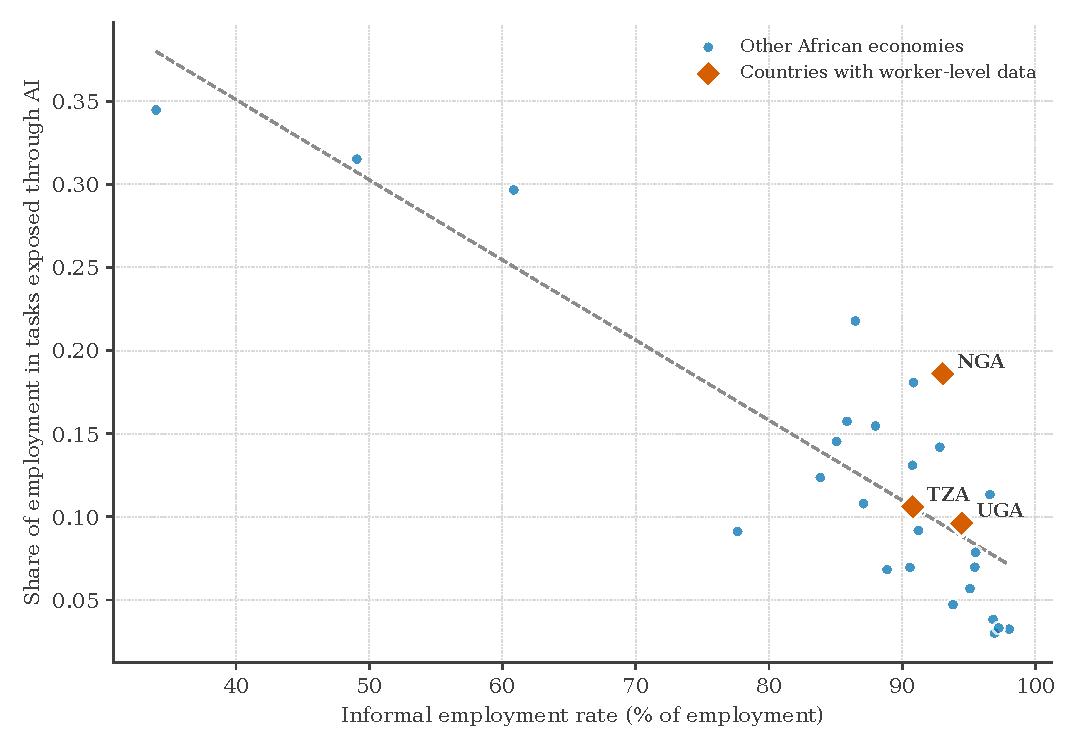
\includegraphics[width=0.8\linewidth]{figures/fig_macro_exposure_informality}
\caption{Share of tasks rated exposed through AI against the informal
employment rate, 28 African economies. The dashed line is a linear fit.}
\label{fig:macro}
\end{figure}

\section{Limitations}

The exposure measure is built outside Africa. It scores the task composition of
US occupations, and it reaches an African worker only through a crosswalk. A
Ugandan shopkeeper and a US retail salesperson share an ISCO code and receive
the same score, though the two jobs differ in tools, scale and what the worker
actually spends the day doing. If African jobs inside a given occupation are
more manual than their US counterparts, the measure overstates exposure here,
and the direction of that bias runs against the paper's finding.

The level of exposure is a property of the version of the measure used. Across
the nine published versions the pooled weighted mean runs from 0.045 to 0.489.
Section~\ref{sec:measure} reports all nine, and every level statement in the
paper is tied to the moderate Qwen scenario.

The occupation coding is uneven. Tanzania codes occupation for non-farm work
only, and its farmers enter through the own-use route. It also asks no
occupation of non-farm business owners without a wage job, which removes 1,789
own-account workers and leaves the pooled own-account figures resting on Nigeria
and Uganda.
Nigeria leaves 65 of the 7,656 people its labour module records as working
without an occupation code. Ethiopia offers only one-digit codes and is reported
separately.

Whether non-agricultural wage or own-account work is more exposed is not settled
here. The gap is 0.016, it falls to zero under the extreme crosswalk bound, and
it reverses under six of the nine versions of the exposure measure.

Uganda's survey supplies no enumeration-area identifier, and the parish stands
in as the primary sampling unit. For 751 of its 3,094 households, tracked movers
and split-offs, and the resulting standard errors
understate clustering. Appendix~\ref{app:design} gives district-level clustering
as a bound, which moves the standard error of Uganda's mean from 0.0017 to
0.0025.

The design is descriptive throughout. We do not identify a causal effect of
occupational structure on exposure, and the cross-country regressions are
associations among 27 country averages, several of which are close to being the
same variable measured differently.

\section{Conclusion}

This paper measures generative-AI task exposure across three Sub-Saharan African
economies with household survey data that distinguish agricultural,
own-account and wage work, record wage-job formality, and also include own-use
producers outside the conventional employment boundary. Exposure is low, spread very unevenly
across occupations, and concentrated in a small set of white-collar jobs, on
the moderate 2030 ratings scored by Qwen 2.5. Agricultural workers, who are
62.2 percent of the pooled sample and 48.6 percent of the weighted population,
average 0.029 against 0.150 for non-agricultural wage employees. Clerical
support, the most exposed major occupational group by a wide margin at 0.615,
employs 0.6 percent of the sample. Across African economies, exposure is
negatively associated with agricultural employment. The strength and
interpretation of that relationship depend on how country exposure is
measured.

Formality tracks exposure inside
wage work, where formal employees score about twice what informal ones do. 
Own-account formality is unmeasured. 
The measured distance between farming and everything else comes
from the task content the measure assigns to farming.

The level of exposure is a property of the measure. Across the nine published
versions of the task ratings the pooled figure moves by a factor of ten. 
Agriculture is the least exposed group
in every version, and far below both non-agricultural groups. Clerical support
is the most exposed major group in eight of the nine and second to managers in
the ninth. Formal wage employees score above informal ones in every one. Nigeria
sits above the other two in every one. Whether wage or own-account work sits 
higher inside non-agricultural employment moves with the
version. And the distance between Uganda and Tanzania is smaller than Tanzania's
own coverage gap, so the country ranking carries Nigeria's distance from the
other two and no more.

And exposure is distinct from displacement. Under the moderate 2030 scenario,
the occupational reach of generative AI in these economies falls
disproportionately on a small share of workers, which says
where the technology could bite first. Whether firms will adopt it, whether
output per worker will rise, and whether anyone will lose a job are separate
questions, and answering them needs data on adoption and outcomes that these
surveys do not have.

\section*{Declaration of generative AI in the
manuscript preparation process}

Statement: During the preparation of this work the author used Claude Opus 5
for code generation and debugging and for prose editing. The author designed
the analysis, independently audited the code, and reproduced all outputs. The
author takes full responsibility for the content of the manuscript.

\bibliographystyle{plainnat}
\bibliography{refs}

\appendix
\section{Source of the task ratings}
\label{app:source}

\begin{sloppypar}
The task ratings come from the public repository that accompanies
\citet{althoff2026}, \url{https://github.com/lukasalthoff/ai_labor_markets}.
The canonical file is \nolinkurl{ai_capabilities/task_ai_capabilities.csv} at
commit \texttt{4706d49} of 7 June 2026, downloaded on 18 September 2026, with
SHA-256 checksum beginning \texttt{b56dcf23dd0a}.
\end{sloppypar}

Each occupation's score is the task-weighted mean of its task ratings,
\[
  s_o = \frac{\sum_{t \in o} w_t a_t}{\sum_{t \in o} w_t},
\]
where $a_t$ is the binary rating of task $t$ (\texttt{automatable\_genai}) and
$w_t$ is its O*NET importance weight (\texttt{task\_weight}). Applied to the
canonical file, this formula reproduces all 974 scores in the published
occupation file to within $10^{-16}$. The eight alternative model and scenario
files reported in Section~\ref{sec:measure} are fixed in the same way. The
replication package records the commit, address, download date and full
checksum of each file in \nolinkurl{countries/althoff_provenance.json}.

\section{Survey variables}
\label{app:vars}

Table~\ref{tab:vars} lists the survey variables behind each harmonised concept.
All come from the public LSMS-ISA release of each wave. In Nigeria the
derived work-status variable (\texttt{s4aq21}) places a person on the family
farm only when that farm is their sole work and its output is only or mainly
for household use, on the answers to the destination questions in the last row.

\begin{table}[ht]
\centering
\caption{Survey variables used for each harmonised concept}
\label{tab:vars}
\footnotesize
\begin{tabular}{llll}
\toprule
Concept & Nigeria 2023 & Tanzania 2020 & Uganda 2019 \\
\midrule
Four-digit occupation      & \texttt{s4aq40\_code}   & \texttt{hh\_e30b\_4a}    & \texttt{h8q19b\_fourDigit} \\
Wage employment            & \texttt{s4aq51}         & \texttt{hh\_e03}         & \texttt{s8q22} \\
Written contract           & \texttt{s4aq56}         & \texttt{hh\_e42}         & \texttt{s8q27} \\
Second formality marker    & \texttt{s4aq57\_\_1}    & \texttt{hh\_e44b}        & \texttt{s8q26} \\
                           & (pension)               & (tax withheld)           & (PAYE) \\
Non-farm business owner    & --                      & \texttt{hh\_e05}         & -- \\
Farm work                  & \texttt{s4aq21}         & \texttt{hh\_e07}         & -- \\
Destination of farm output & \texttt{s4aq13a}--\texttt{c}, & \texttt{hh\_e09}   & -- \\
                           & \texttt{s4aq19a}--\texttt{b}  &                    &    \\
Household weight           & \texttt{wt\_cross\_wave5} & \texttt{y5\_crossweight} & \texttt{wgt} \\
\bottomrule
\end{tabular}

\vspace{4pt}
\begin{minipage}{0.9\linewidth}
\footnotesize
Nigeria's variables are in the post-harvest labour module (\texttt{sect4a})
and household cover file (\texttt{secta}), Tanzania's in \texttt{hh\_sec\_e1}
and \texttt{hh\_sec\_a}, and Uganda's in \texttt{gsec8} and \texttt{gsec1}.
In Nigeria the destination questions refer to the last seven days
(\texttt{s4aq13a}--\texttt{c}) or, for people with no farm work that week, to
usual farm work (\texttt{s4aq19a}--\texttt{b}). A dash marks a concept the
survey does not use for this purpose.
\end{minipage}
\end{table}

\section{Ethiopia}
\label{app:ethiopia}

The Ethiopian Socioeconomic Panel Survey Wave 5 records occupation at the
one-digit ISCO-88 major group, which cannot support the occupational argument
of this paper. Ethiopia is therefore reported here and left out of the headline
sample.

Two Ethiopian samples exist in the survey. The first holds 584 out-migrants,
household members who had left and whose occupation the household reported.
That sample is a poor description of the Ethiopian workforce, with an
agricultural share of 22.4 percent against a national figure above 60 percent,
and it is left aside here. The resident wage sample is the better object. It holds 1,989
workers with a one-digit code, mapped to ISCO-08 exposure through the unit-group
correspondence.

Resident Ethiopian wage workers average 0.216, weighted 0.190. Of them, 37.1
percent have no written contract, 45.9 percent on weights, and those workers
average 0.129 against 0.267 for workers with a contract. The formal-informal
ratio is close to the one found in the three headline countries. The sample
covers wage jobs only and can say nothing about agriculture or own-account work,
which is why it supplements the main analysis and does not enter it.

\section{Cross-country detail}
\label{app:macro}

Table~\ref{tab:macro} in the body reports one Atlas outcome and one ILOSTAT
score vector. Four Atlas outcomes are available. They are the total exposed
share, the share exposed through AI, the share exposed through learned content
transformation, and the share exposed with no AI involved. Informality carries a
large full-model coefficient on the first three and $-0.006$ with a standard
error of 0.034 on the fourth, which cannot be told from zero. That is the basis
for the claim in Section 6 that the Atlas informality result is a property of
its AI classification.

\begin{table}[ht]
\centering
\caption{Atlas outcomes, full model}
\label{tab:atlas}
\small
\begin{tabular}{lrrrrr}
\toprule
Outcome & African & Informality & Informality & Agricultural & Log GDP \\
        & median  & alone       & full model  & self-emp.    & per head \\
\midrule
Exposed, any route            & 0.242 & $-0.617$ & $-0.248$ & $-0.113$ & 0.077 \\
                              &       & (0.077)  & (0.068)  & (0.074)  & (0.015) \\
Exposed through AI            & 0.107 & $-0.482$ & $-0.242$ & $-0.093$ & 0.045 \\
                              &       & (0.046)  & (0.049)  & (0.048)  & (0.011) \\
Exposed, content transf.      & 0.068 & $-0.220$ & $-0.087$ & $-0.058$ & 0.023 \\
                              &       & (0.029)  & (0.029)  & (0.028)  & (0.006) \\
Exposed, no AI                & 0.132 & $-0.134$ & $-0.006$ & $-0.020$ & 0.032 \\
                              &       & (0.034)  & (0.034)  & (0.032)  & (0.007) \\
\bottomrule
\end{tabular}

\vspace{4pt}
\begin{minipage}{0.94\linewidth}
\footnotesize
32 African economies; each model uses the countries reporting its covariates, 28
to 31. Heteroskedasticity-robust standard errors in parentheses. The agricultural
self-employment and income coefficients are from the full model, which holds all
three variables at once.
\end{minipage}
\end{table}

Table~\ref{tab:macro} reports the three predictors on their own scales, two of
them shares and one a logarithm. Nothing in it ranks them.
Table~\ref{tab:fit} puts them on a common footing. Standardised coefficients
multiply each coefficient by the ratio of the predictor's standard deviation to
the outcome's. Incremental R-squared is what the full model loses when that one
predictor is dropped. Both run on the 27 countries where both outcomes and all
three predictors are present, with the same HC1 errors as
Table~\ref{tab:macro}.

The two measures disagree about which predictor leads. Under the ILOSTAT
rebuild the agricultural share is first on both metrics. Under the Atlas
measure income per head has the largest standardised coefficient while
informality has the larger incremental R-squared, and the two are close enough
that neither leads.

\begin{table}[ht]
\centering
\caption{Comparable predictor metrics for the two country measures}
\label{tab:fit}
\small
\begin{tabular}{lrrrr}
\toprule
 & \multicolumn{2}{c}{Atlas, exposed through AI} & \multicolumn{2}{c}{ILOSTAT rebuild} \\
\cmidrule(lr){2-3}\cmidrule(lr){4-5}
Predictor & Std. coef. & Incr. $R^2$ & Std. coef. & Incr. $R^2$ \\
\midrule
Informal employment rate     & $-0.401$ & 0.085 & $-0.182$ & 0.018 \\
Agricultural self-employment & $-0.240$ & 0.030 & $-0.492$ & 0.124 \\
Log GDP per head             & 0.406    & 0.077 & 0.301    & 0.043 \\
\midrule
Countries                    & \multicolumn{2}{c}{27} & \multicolumn{2}{c}{27} \\
Full-model $R^2$             & \multicolumn{2}{c}{0.837} & \multicolumn{2}{c}{0.740} \\
\bottomrule
\end{tabular}

\vspace{4pt}
\begin{minipage}{0.94\linewidth}
\footnotesize
Both columns use the full model of Table~\ref{tab:macro}, which holds all three
predictors at once, on the 27 countries where both outcomes and all three
predictors are present. Standardised coefficients are the unstandardised
coefficient times the predictor's standard deviation over the outcome's.
Incremental R-squared is the full-model R-squared less the R-squared of the
model without that predictor. Heteroskedasticity-robust standard errors as in
Table~\ref{tab:macro}. The unstandardised coefficients reproduce
Table~\ref{tab:macro} on its own per-specification samples, 28 countries for
the Atlas outcome and 27 for the ILOSTAT rebuild.
\end{minipage}
\end{table}

The ILOSTAT rebuild covers 45 African countries. Central African Republic, Libya
and Mauritania report no data; Eritrea, South Sudan and South Africa report only
ISCO-88; Algeria and Morocco carry no ISCO-08 series from 2015. Armed forces and
unclassified workers are excluded and the shares rescaled over groups 1 to 9.
Three score vectors give country medians of 0.123 (the mean over ISCO-08 unit
codes), 0.088 (the survey-weighted worker scores) and 0.095 (the survey scores
with own-use farmers excluded). The three rank countries almost identically,
correlating at 0.98 or above, and the reported results hold under all three.
Excluding the four countries with more than 20 percent of workers unclassified
leaves the same pattern on 25 countries.

\section{Survey design}
\label{app:design}

Table~\ref{tab:design} gives the sampling design used for the standard errors
reported throughout the paper.

\begin{table}[ht]
\centering
\caption{Sampling design by country}
\label{tab:design}
\small
\begin{tabular}{llrrr}
\toprule
Country & Primary sampling unit & PSUs & Strata & Fewest PSUs \\
        &                       &      &        & in a stratum \\
\midrule
Nigeria       & Survey cluster          & 731 & 6  & 103 \\
Tanzania      & Survey cluster          & 485 & 55 & 2 \\
Uganda        & Parish (2018 codes)     & 930 & 7  & 4 \\
Ethiopia      & Enumeration area        & 314 & 19 & 6 \\
\bottomrule
\end{tabular}

\vspace{4pt}
\begin{minipage}{0.94\linewidth}
\footnotesize
Strata are the survey's own where supplied. For Uganda they are Kampala, other
urban, and rural by region. Tanzania's 545 booster households, added outside the
2014/15 frame, form one stratum per city with their enumeration area as the
primary sampling unit; Tanga urban has a single such unit and joins Tanga rural.
Ethiopia is the resident wage sample of Appendix~\ref{app:ethiopia}.
\end{minipage}
\end{table}

Uganda's design needs a caveat. The survey samples through enumeration areas,
and no household file carries an enumeration-area code. The parish stands in.
Of the 3,094 households with parish codes, 2,343 live in one of the 296 parishes
covered by the community survey. The other 751, tracked movers and split-offs,
sit alone or nearly alone in their parish and each counts as its own primary
sampling unit, which understates clustering. Clustering Uganda more coarsely
moves the standard error of its mean from 0.0017 at parish level to 0.0018 at
subcounty, 0.0020 at county and 0.0025 at district. The standard errors of
Uganda's status-group means move by 0.0007 or less, some of them downward. The
district figure is the honest upper bound.

Across the 35 group means, standard errors that allow for strata and clusters run from 0.96 to 1.55
times their household-clustered counterparts. The ratio is largest for groups
whose members share villages, at 1.55 for Nigeria's farmers, and close to one
for clerical support and formal wage workers, who are scattered thinly across
clusters.
